\documentclass[conference,a4paper]{IEEEtran}

\usepackage[T1]{fontenc}
\usepackage[utf8]{inputenc}
\usepackage{amsmath,amssymb,amsfonts}
\usepackage{graphicx}
\usepackage{booktabs}
\usepackage{algorithm}
\usepackage{algpseudocode}
\usepackage[nocompress]{cite}
\usepackage{xcolor}
\usepackage{url}
\usepackage[hidelinks]{hyperref}

% IEEEtran puts an em dash after "Abstract" and "Index Terms"; these blocks use a colon instead.
\makeatletter
\newenvironment{plainabstract}{\par\noindent\small\bfseries\textit{Abstract:}\ \ignorespaces}{\par\medskip}
\newenvironment{plainkeywords}{\par\noindent\small\bfseries\textit{Index Terms:}\ \ignorespaces}{\par\medskip}
\makeatother

\graphicspath{{figures/}{logos/}}

\newcommand{\R}{\mathbb{R}}
\newcommand{\norm}[1]{\lVert #1\rVert}
\newcommand{\TV}{\mathrm{TV}}
\DeclareMathOperator{\diag}{diag}
\DeclareMathOperator{\clip}{clip}
\algrenewcommand\algorithmicrequire{\textbf{Input:}}

\begin{document}

\title{%
  \vspace*{-9mm}%
  \makebox[\textwidth]{
\includegraphics[height=9mm]{etf}\hfill
\includegraphics[height=9mm]{dsai}}\\[-1mm]
  \rule{\textwidth}{0.4pt}\\[5mm]
  Total Variation Image Denoising with Gradient Descent and a Newton-Type Lagged Diffusivity Method}

\author{\IEEEauthorblockN{Kemal Sivro, Student ID 20015}
\IEEEauthorblockA{Faculty of Electrical Engineering, University of Sarajevo, Bosnia and Herzegovina\\
Seminar paper in Numerical Optimisations, Data Science and Artificial Intelligence\\
Professor: Izudin Džafić, academic year 2025/26\\
Source code: \url{https://github.com/vrosi21/TV-Image-Denoising}}}

\maketitle

\begin{plainabstract}
Total variation denoising recovers an image by minimising the sum of a quadratic data term and a weighted total variation of the image. This paper compares two solvers for a smoothed version of this model, both implemented in C++ on the natID framework and run on identical seeded noise: gradient descent with Armijo backtracking, and a Newton-type method that solves one sparse linear system per iteration, known as the lagged diffusivity or iteratively reweighted least squares method. On three $225\times225$ test images with noise level $\sigma=0.1$ and $\lambda=0.1$, both methods reach the same image quality. Gradient descent costs 3.5 to 5.3\,ms per iteration and reaches its best peak signal-to-noise ratio (PSNR) within 4 to 40 iterations; the Newton-type method costs 101 to 123\,ms per iteration, reaches its best PSNR within 2 to 5 iterations and reduces the relative change of the iterate by a factor of ten or more every ten iterations. Its smoothing parameter introduces a bias: its limit has a 0.9 to 1.7\% higher exact TV energy than gradient descent after 300 iterations. At the PSNR-optimal $\lambda$ both methods agree within 0.08\,dB. A scaling study shows that the dense Newton system grows like $N^3$ and reaches 1.6\,s per iteration at $N=4096$ pixels, while the sparse $LDL^\top$ path grows almost linearly and needs 0.5\,s at $N=202{,}500$.
\end{plainabstract}

\begin{plainkeywords}
total variation, image denoising, gradient descent, Armijo line search, Newton method, lagged diffusivity, sparse Cholesky
\end{plainkeywords}

\section{Introduction}

Noise removal that preserves edges is a basic task in image processing. The model of Rudin, Osher and Fatemi \cite{rudin1992} achieves this by penalising the total variation of the image: smooth noise-like oscillations have a large total variation, while a sharp edge of a given height costs no more than a gradual ramp. The resulting problem is convex, so it has a unique minimiser, but the total variation is not differentiable where the image gradient vanishes. Practical methods either smooth the functional \cite{vogel1996}, work with a dual formulation \cite{chambolle2004} or use primal-dual splitting \cite{chambolle2011,beck2009}.

This work studies the smoothed approach, because it allows a direct comparison of a first-order and a second-order method on the same objective. The contributions are:
\begin{itemize}
\item an implementation of gradient descent with Armijo backtracking and of the lagged diffusivity Newton-type method, with a dense and a sparse linear solver;
\item a comparison on three standard images in terms of PSNR, exact TV energy, relative change and wall time, together with studies of the regularisation weight $\lambda$, the smoothing parameter $\varepsilon$ and the noise level;
\item a scaling study of the cost per iteration from 64 to 202{,}500 pixels;
\item a cross-platform desktop application that runs every experiment interactively.
\end{itemize}

Section~\ref{sec:model} states the model, Section~\ref{sec:methods} the two methods and Section~\ref{sec:impl} the implementation. Results follow in Section~\ref{sec:results} and are discussed in Section~\ref{sec:discussion}.

\section{Model}\label{sec:model}

\subsection{Discrete total variation}

Let $f\in[0,1]^{H\times W}$ be the observed image and $N=HW$. Forward differences with a zero difference at the last column and row define
\begin{align}
(D_xu)_{i,j}&=\begin{cases}u_{i,j+1}-u_{i,j}, & j<W,\\ 0, & j=W,\end{cases}\label{eq:dx}\\
(D_yu)_{i,j}&=\begin{cases}u_{i+1,j}-u_{i,j}, & i<H,\\ 0, & i=H,\end{cases}\label{eq:dy}
\end{align}
and the discrete gradient $D=\bigl[\begin{smallmatrix}D_x\\D_y\end{smallmatrix}\bigr]\in\R^{2N\times N}$. The isotropic total variation and its smoothed version are
\begin{align}
\TV(u)&=\sum_{i,j}\sqrt{(D_xu)_{i,j}^2+(D_yu)_{i,j}^2},\label{eq:tv}\\
\TV_\varepsilon(u)&=\sum_{i,j}\sqrt{(D_xu)_{i,j}^2+(D_yu)_{i,j}^2+\varepsilon^2},\qquad\varepsilon>0.\label{eq:tveps}
\end{align}
The function $\sqrt{t^2+\varepsilon^2}$ behaves like $|t|$ for $|t|\gg\varepsilon$ and like a quadratic near zero, similar to the Huber function \cite{huber1964}; the application therefore calls it Huber smoothing.

\subsection{Objective}

The denoised image minimises
\begin{equation}
F_\varepsilon(u)=\frac12\norm{u-f}_2^2+\lambda\,\TV_\varepsilon(u),
\label{eq:objective}
\end{equation}
where $\lambda>0$ balances noise removal against fidelity. Because the data term is 1-strongly convex and $\TV_\varepsilon$ is convex, $F_\varepsilon$ has a unique minimiser for every $\varepsilon\ge0$. The solvers minimise $F_\varepsilon$, but for a fair comparison all reported energies use the exact functional $E(u)=\frac12\norm{u-f}^2+\lambda\TV(u)$, i.e.\ $\varepsilon=0$. Quality is measured against the clean image $u^\circ$ by
\begin{equation}
\mathrm{PSNR}(u)=10\log_{10}\frac{1}{\mathrm{MSE}},\qquad \mathrm{MSE}=\frac1N\norm{u-u^\circ}_2^2.
\label{eq:psnr}
\end{equation}

\subsection{Derivatives}

With the per-pixel weights
\begin{equation}
w_{i,j}(u)=\Bigl((D_xu)_{i,j}^2+(D_yu)_{i,j}^2+\varepsilon^2\Bigr)^{-1/2}
\label{eq:weights}
\end{equation}
and $W(u)=\diag(w,w)\in\R^{2N\times2N}$, the gradient is
\begin{equation}
\nabla F_\varepsilon(u)=u-f+\lambda\,D^\top W(u)\,D\,u.
\label{eq:gradient}
\end{equation}
Written per pixel, with $d^x=D_xu$ and $d^y=D_yu$,
\begin{multline}
\bigl[D^\top WDu\bigr]_{i,j}=-w_{i,j}\bigl(d^x_{i,j}+d^y_{i,j}\bigr)\\
+w_{i,j-1}\,d^x_{i,j-1}+w_{i-1,j}\,d^y_{i-1,j},
\label{eq:divergence}
\end{multline}
with terms outside the image set to zero. This is the negative discrete divergence of $\nabla u/|\nabla u|_\varepsilon$.

Differentiating once more gives the Hessian
\begin{equation}
\nabla^2F_\varepsilon(u)=I+\lambda\,D^\top B(u)\,D,
\label{eq:hessian}
\end{equation}
where $B(u)$ consists of one $2\times2$ block per pixel,
\begin{equation}
B_{i,j}=\frac{1}{r}\,I_2-\frac{1}{r^3}\begin{bmatrix}d^x\\d^y\end{bmatrix}\begin{bmatrix}d^x & d^y\end{bmatrix},\qquad r=\frac{1}{w_{i,j}}.
\label{eq:hessblock}
\end{equation}
The eigenvalues of $B_{i,j}$ are $1/r$ and $\varepsilon^2/r^3$, so $0\prec B(u)\preceq W(u)$ and
\begin{equation}
I\preceq\nabla^2F_\varepsilon(u)\preceq A(u)=I+\lambda\,D^\top W(u)\,D.
\label{eq:bounds}
\end{equation}
Since $\norm{D}_2^2\le8$ and $w\le1/\varepsilon$, the gradient \eqref{eq:gradient} is Lipschitz continuous with constant
\begin{equation}
L\le1+\frac{8\lambda}{\varepsilon},
\label{eq:lipschitz}
\end{equation}
so the condition number of $F_\varepsilon$ can be as large as $1+8\lambda/\varepsilon$.

\section{Methods}\label{sec:methods}

\subsection{Gradient descent with Armijo backtracking}

Each iteration computes $g_k=\nabla F_\varepsilon(u_k)$ and finds a step length $t$ by backtracking from $t=1$ with factor $\beta=\frac12$ until the Armijo condition \cite{armijo1966}
\begin{equation}
F_\varepsilon(u_k-t\,g_k)\le F_\varepsilon(u_k)-\alpha\,t\,\norm{g_k}_2^2,\qquad\alpha=0.01,
\label{eq:armijo}
\end{equation}
holds, with at most 40 reductions. The update is projected onto the valid pixel range,
\begin{equation}
u_{k+1}=\clip\bigl(u_k-t\,g_k,\,0,\,1\bigr).
\label{eq:gdupdate}
\end{equation}
The implementation fixes $\varepsilon=10^{-3}$ for gradient descent. With \eqref{eq:lipschitz}, $\lambda=0.1$ gives $L\le801$, and backtracking accepts steps of order $1/L$. Convergence is linear with a rate that depends on $L$ \cite{nocedal2006,boyd2004}: components of the error along directions of large curvature, such as pixel-scale oscillations, are removed in a few iterations, while smooth components decay slowly.

\subsection{Newton-type lagged diffusivity method}

A full Newton step would use \eqref{eq:hessian}. The lagged diffusivity method \cite{vogel1996} instead freezes the weights at the current iterate and uses the matrix $A(u_k)$ from \eqref{eq:bounds}. Because \eqref{eq:gradient} can be written as $\nabla F_\varepsilon(u)=A(u)\,u-f$, the Newton-type step with this matrix is
\begin{equation}
u_{k+1}=u_k-A(u_k)^{-1}\nabla F_\varepsilon(u_k)=A(u_k)^{-1}f,
\label{eq:irls}
\end{equation}
so each iteration solves one symmetric positive definite system
\begin{equation}
\bigl(I+\lambda D^\top W(u_k)D\bigr)\,u_{k+1}=f.
\label{eq:system}
\end{equation}
This is also an iteratively reweighted least squares (IRLS) step, since $u_{k+1}$ minimises the weighted quadratic $\frac12\norm{u-f}^2+\frac\lambda2\sum w_{i,j}(u_k)|(Du)_{i,j}|^2$.

The iteration decreases $F_\varepsilon$ monotonically. The function $s\mapsto\sqrt{s+\varepsilon^2}$ is concave, so for every pixel $\sqrt{s+\varepsilon^2}\le\sqrt{s_0+\varepsilon^2}+\frac{w_0}{2}(s-s_0)$. Summing over pixels shows that
\begin{equation}
G(v;u)=\frac12\norm{v-f}^2+\frac\lambda2\sum_{i,j}w_{i,j}(u)\,|(Dv)_{i,j}|^2+c(u)
\label{eq:majorizer}
\end{equation}
satisfies $G(v;u)\ge F_\varepsilon(v)$ and $G(u;u)=F_\varepsilon(u)$. The step \eqref{eq:irls} minimises $G(\cdot;u_k)$, hence $F_\varepsilon(u_{k+1})\le G(u_{k+1};u_k)\le G(u_k;u_k)=F_\varepsilon(u_k)$. Global convergence of the method was proved by Chan and Mulet \cite{chan1999mulet}. Its rate is linear, not quadratic, because the curvature term in \eqref{eq:hessblock} is ignored; primal-dual Newton methods recover it \cite{chan1999primaldual}. The implementation clips $u_{k+1}$ to $[0,1]$ as in \eqref{eq:gdupdate} and exposes $\varepsilon$ to the user, with default $10^{-2}$.

\begin{algorithm}[t]
\caption{Lagged diffusivity (Newton-type) iteration}\label{alg:irls}
\begin{algorithmic}[1]
\Require noisy image $f$, $\lambda$, $\varepsilon$, iterations $K$
\State $u\gets f$
\For{$k=1,\dots,K$}
  \State compute $w_{i,j}(u)$ by \eqref{eq:weights}
  \State assemble $A=I+\lambda D^\top W D$ \Comment{five nonzeros per row}
  \If{$N\le4096$} solve $Au_{\mathrm{new}}=f$ by dense LU
  \Else\ solve $Au_{\mathrm{new}}=f$ by sparse $LDL^\top$
  \EndIf
  \State $u\gets\clip(u_{\mathrm{new}},0,1)$
\EndFor
\end{algorithmic}
\end{algorithm}

\subsection{Linear algebra}

In row-major pixel order $A(u)$ has at most five nonzeros per row:
\begin{align}
A_{k,k}&=1+\lambda\bigl(w_k[j<W]+w_{k-1}[j>1]\nonumber\\
&\qquad+w_k[i<H]+w_{k-W}[i>1]\bigr),\label{eq:diag}\\
A_{k,k-1}&=-\lambda\,w_{k-1},\qquad A_{k,k-W}=-\lambda\,w_{k-W},\label{eq:offdiag}
\end{align}
where $k$ is the index of pixel $(i,j)$ and $[\cdot]$ is 1 when the condition holds. For $N\le4096$ the system is assembled as a dense matrix and solved with the LU solver of the natID matrix library, which costs $O(N^2)$ memory and $O(N^3)$ time. A dense matrix for a $225\times225$ image would need $N^2=2.6\times10^9$ entries, about 20\,GB, so larger images use the sparse $LDL^\top$ solver of natID with its own fill-reducing ordering. For regular grids, nested dissection orderings bound the fill to $O(N\log N)$ and the factorisation work to $O(N^{3/2})$ \cite{george1973,davis2006}.

\section{Implementation}\label{sec:impl}

The application is written in C++20 with the natID framework \cite{natid}, which provides the user interface, the dense and sparse matrix libraries and the installer tooling. A GitHub Actions pipeline builds installers for Windows, macOS on Apple Silicon and Intel, and Linux; the code contains no platform-specific calls.

\subsection{Design}

The numerical classes do not depend on the user interface. \texttt{ImageData} stores a grayscale image as 32-bit floating point values in $[0,1]$, loads PNG and JPEG files through natID and adds reproducible noise $f=\clip(u^\circ+\sigma z,0,1)$, where $z$ comes from the Mersenne Twister with a hand-written Box-Muller transform, so a seed gives identical noise on every platform. Both solvers implement the interface \texttt{ITVSolver}, whose \texttt{denoise} method accepts an observer called after every iteration; the observer records metrics and delivers cancellation, so the solvers contain no measurement or threading code. \texttt{DenoisingMetrics} computes $E(u)$, PSNR and the relative change, and \texttt{DenoisingRunner} executes a comparison or a $\lambda$ study without any user interface, on a background thread in the application and from a console program in this paper.

\subsection{Application}

Fig.~\ref{fig:gui} shows the main window. The sidebar selects the image and holds sliders for $\sigma$, $\lambda$, $\varepsilon$ and the number of iterations, the seed, the methods to run and the range of the $\lambda$ study. The \emph{Overview} tab shows one card per method with the PSNR, gain, iterations and time, marks the best and fastest method, and displays the images in the arrangement that makes them largest. The \emph{Convergence} tab plots the exact energy gap, the PSNR and the relative change per iteration and the PSNR against wall time; the \emph{Lambda study} tab plots PSNR against $\lambda$, the L-curve and the cost; \emph{Report} lists all numbers and \emph{Log} records the session. Runs can be stopped and optionally repeat on every change. Charts are exported as PDF or SVG, images as PNG and data as CSV into a time-stamped folder.

\begin{figure}[t]
\centering
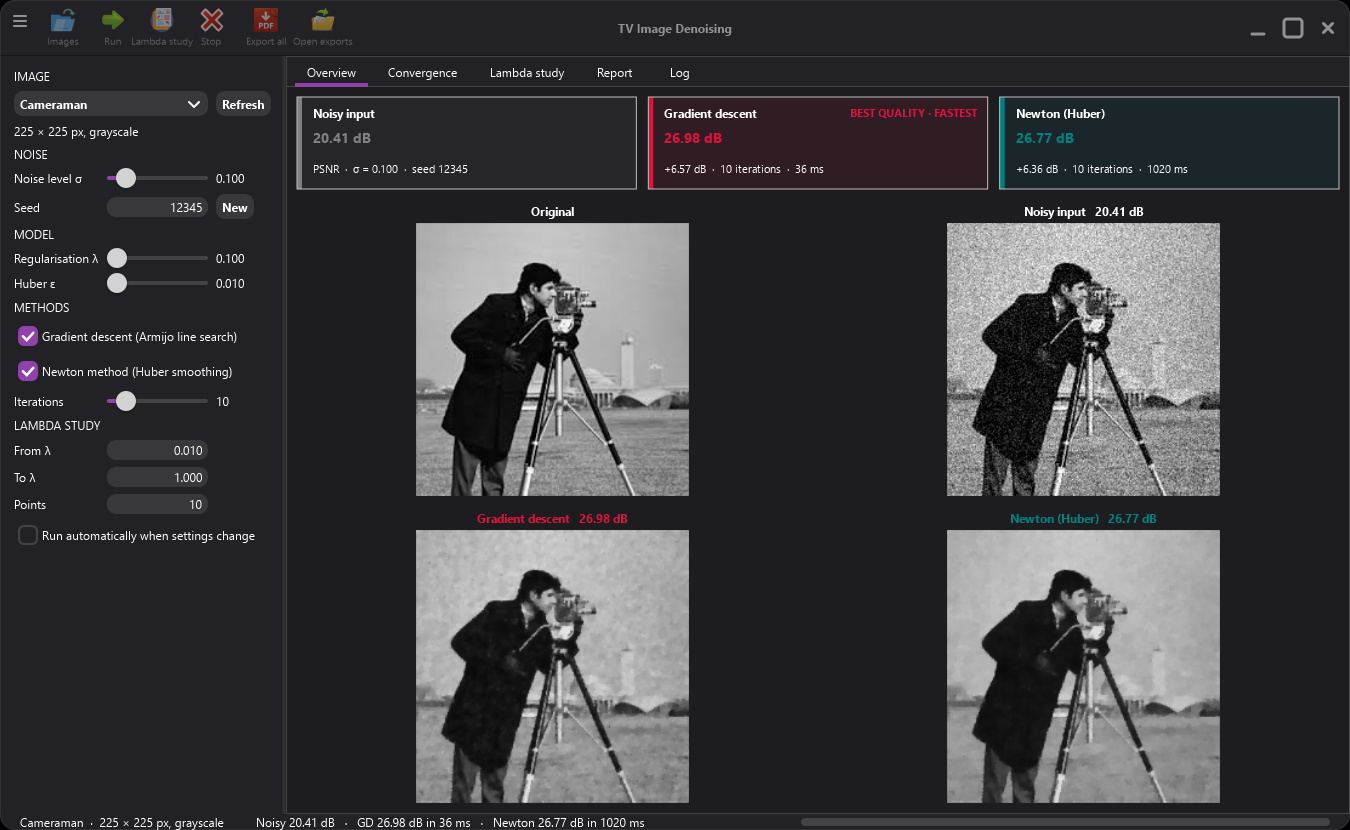
\includegraphics[width=\columnwidth]{gui}
\caption{Overview tab after a comparison on Cameraman with $\sigma=0.1$, $\lambda=0.1$, $\varepsilon=0.01$ and 10 iterations.}
\label{fig:gui}
\end{figure}

\section{Results}\label{sec:results}

All experiments were run by a console program that compiles the solver classes of the application without changes, on an Intel Core i5-1345U with 32\,GB of memory under Windows 11 (MSVC, Release build). The test images Cameraman, Barbara and Ape have $225\times225$ pixels. Unless stated otherwise $\sigma=0.1$ with seed 12345, $\lambda=0.1$, $\varepsilon=10^{-3}$ for gradient descent (GD) and $\varepsilon=10^{-2}$ for the Newton-type method (NT). GD ran 300 and NT 30 iterations.

\subsection{Quality and convergence}

\begin{figure*}[t]
\centering
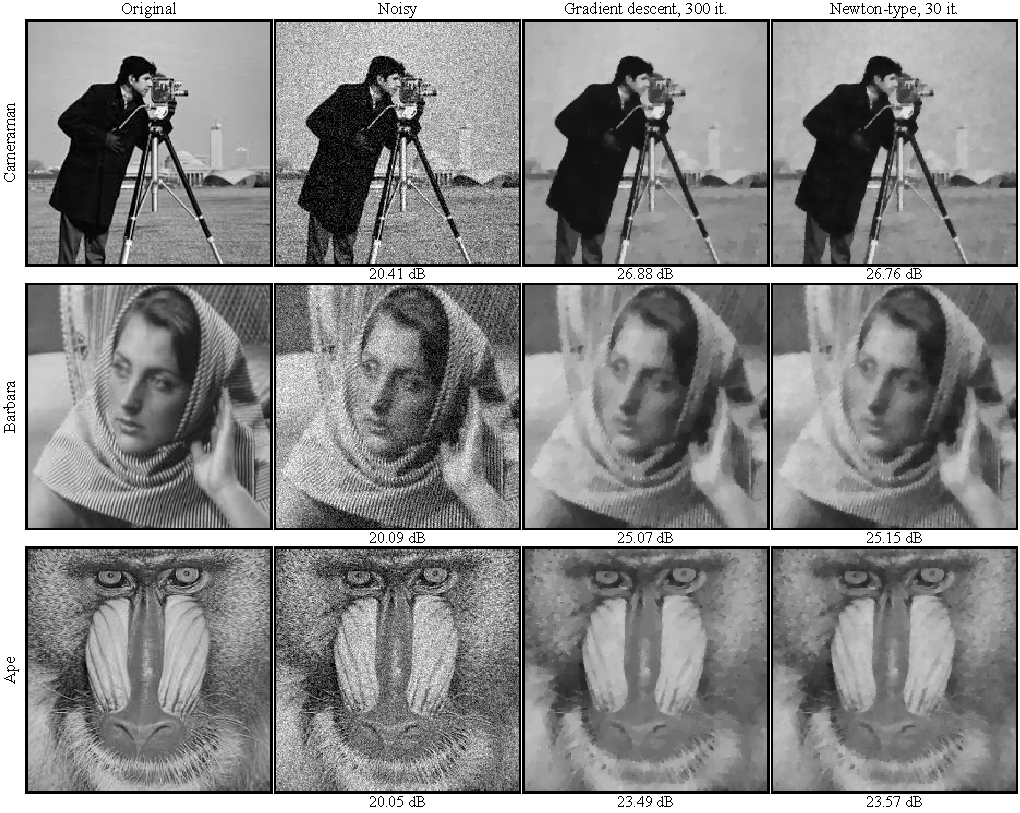
\includegraphics[width=0.92\textwidth]{gallery}
\caption{Test images, noisy input ($\sigma=0.1$) and results of both methods with $\lambda=0.1$. Numbers are PSNR values.}
\label{fig:gallery}
\end{figure*}

\begin{table*}[t]
\caption{Comparison at $\sigma=0.1$, $\lambda=0.1$. Best: highest PSNR over all iterations (iteration in brackets). $E$: exact TV energy of the final iterate. Time: mean wall time per iteration.}\label{tab:comparison}
\centering
\small
\begin{tabular}{@{}lr ccccr ccccr@{}}
\toprule
& & \multicolumn{5}{c}{Gradient descent, $\varepsilon=10^{-3}$} & \multicolumn{5}{c}{Newton-type, $\varepsilon=10^{-2}$}\\
\cmidrule(lr){3-7}\cmidrule(l){8-12}
Image & Noisy & Best & $k=10$ & $k=300$ & $E$ & ms/it. & Best & $k=10$ & $k=30$ & $E$ & ms/it.\\
\midrule
\csname @@input\endcsname figures/table_comparison.tex
\bottomrule
\end{tabular}
\end{table*}

Fig.~\ref{fig:gallery} shows the results and Table~\ref{tab:comparison} the numbers. Both methods raise the PSNR by 3.4 to 6.5\,dB and produce visually similar images with the piecewise constant regions typical of TV denoising; fine texture such as the stripes on Barbara's scarf and the fur of Ape is partly removed. After the application default of 10 iterations GD is ahead on all three images, by up to 0.44\,dB on Ape.

\begin{figure}[t]
\centering
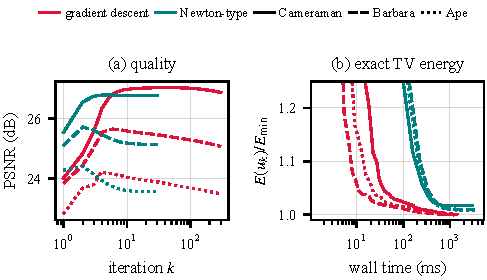
\includegraphics[width=\columnwidth]{convergence}
\caption{(a) PSNR per iteration. (b) Exact TV energy against wall time, relative to the lowest energy observed for the image.}
\label{fig:convergence}
\end{figure}

Fig.~\ref{fig:convergence}(a) shows that the PSNR peaks early and then decreases. GD reaches its best value after 40 iterations on Cameraman, 6 on Barbara and 4 on Ape; NT after 5, 2 and 2 iterations. With $\lambda=0.1$ the minimiser smooths more than the PSNR-optimal solution (Section~\ref{sec:lambda}), so iterates that are not yet converged are closer to the clean image than the minimiser itself.

In terms of the objective, Fig.~\ref{fig:convergence}(b), GD reaches an energy within 2\% of the lowest observed value after 18 to 33 iterations (36 to 136\,ms) and within 1\% after 47 to 65 iterations. NT needs only 5 to 7 iterations for 2\%, but these take 555 to 583\,ms. Its energy then levels off 1.7\% (Cameraman), 1.0\% (Barbara) and 0.9\% (Ape) above the GD result, because it minimises $F_\varepsilon$ with a ten times larger $\varepsilon$.

\begin{figure}[t]
\centering
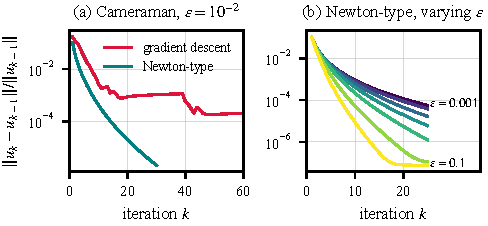
\includegraphics[width=\columnwidth]{rates}
\caption{Relative change $\norm{u_k-u_{k-1}}/\norm{u_{k-1}}$. (a) Both methods on Cameraman. (b) Newton-type method for $\varepsilon\in\{1,2,5\}\times10^{-3}$, $\{1,2,5\}\times10^{-2}$ and $10^{-1}$, dark to light.}
\label{fig:rates}
\end{figure}

The iterates behave differently, as Fig.~\ref{fig:rates}(a) shows. The relative change of NT falls by a factor of ten or more every ten iterations on all images, to $2.1\times10^{-6}$ to $4.0\times10^{-6}$ after 30 iterations, which is the linear convergence expected from Section~\ref{sec:methods}. The relative change of GD is not monotone, because the accepted step length changes between iterations, and after 20 iterations it decreases only slowly, from about $10^{-3}$ to between $3.1\times10^{-5}$ and $1.2\times10^{-4}$ at $k=300$.

\subsection{Smoothing parameter}

\begin{figure}[t]
\centering
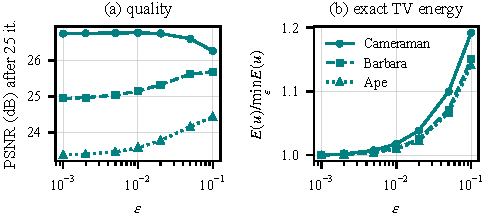
\includegraphics[width=\columnwidth]{epsilon}
\caption{Newton-type method after 25 iterations for different $\varepsilon$. (a) PSNR. (b) Exact TV energy relative to the smallest value over $\varepsilon$.}
\label{fig:epsilon}
\end{figure}

Fig.~\ref{fig:epsilon} and Fig.~\ref{fig:rates}(b) vary $\varepsilon$ for NT. A larger $\varepsilon$ makes the weights \eqref{eq:weights} more uniform and the problem better conditioned: after 25 iterations the relative change is $5.6\times10^{-5}$ to $8.6\times10^{-5}$ for $\varepsilon=10^{-3}$ but $7.6\times10^{-8}$ to $7.8\times10^{-8}$ for $\varepsilon=10^{-1}$, where it is limited by the 32-bit pixel values. The price is a larger bias: from $\varepsilon=10^{-3}$ to $10^{-1}$ the exact energy of the result increases by 19\% on Cameraman, 15\% on Barbara and 14\% on Ape. The PSNR responds differently per image. On Cameraman it stays at 26.74 to 26.76\,dB up to $\varepsilon=0.02$ and drops to 26.26\,dB at $0.1$. On the textured images it increases with $\varepsilon$, by 0.74\,dB on Barbara and 1.07\,dB on Ape, because a large $\varepsilon$ penalises small gradients quadratically and removes less texture, which partly compensates for the too large $\lambda$.

\subsection{Regularisation weight}\label{sec:lambda}

\begin{figure}[t]
\centering
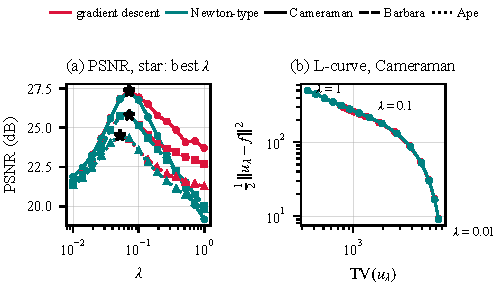
\includegraphics[width=\columnwidth]{lambda}
\caption{Study over 15 logarithmically spaced values $\lambda\in[0.01,1]$ with 200 GD and 20 NT iterations. (a) PSNR, the star marks the best $\lambda$. (b) L-curve for Cameraman.}
\label{fig:lambda}
\end{figure}

Fig.~\ref{fig:lambda} repeats both methods for 15 values of $\lambda$. The best value is $\lambda=0.072$ for Cameraman and Barbara and $0.052$ for Ape, all below the default $0.1$. At the best $\lambda$ the methods agree within 0.08\,dB: 27.39 and 27.31\,dB on Cameraman, 25.80 and 25.83\,dB on Barbara, 24.49 and 24.53\,dB on Ape for GD and NT. For $\lambda$ above the optimum the curves separate. At $\lambda=1$, 200 GD iterations leave the total variation of Cameraman at 752, while NT reaches 344; by \eqref{eq:lipschitz} the Lipschitz constant grows to 8001, so GD takes ten times shorter steps and is far from converged. Its higher PSNR there is again an effect of early stopping. On the L-curve both methods lie on the same curve.

\begin{table}[t]
\caption{Best $\lambda$ on an 11-point grid in $[0.01,1]$ and best PSNR (dB) of GD and NT for several noise levels}\label{tab:sigma}
\centering
\scriptsize
\setlength{\tabcolsep}{1.6pt}
\begin{tabular}{@{}c cccc cccc cccc@{}}
\toprule
& \multicolumn{4}{c}{Cameraman} & \multicolumn{4}{c}{Barbara} & \multicolumn{4}{c}{Ape}\\
\cmidrule(lr){2-5}\cmidrule(lr){6-9}\cmidrule(l){10-13}
$\sigma$ & Noisy & $\lambda^\ast$ & GD & NT & Noisy & $\lambda^\ast$ & GD & NT & Noisy & $\lambda^\ast$ & GD & NT\\
\midrule
\csname @@input\endcsname figures/table_sigma.tex
\bottomrule
\end{tabular}
\end{table}

Table~\ref{tab:sigma} extends the study to four noise levels. The best $\lambda$ grows with the noise, from 0.016 to 0.025 at $\sigma=0.05$ to 0.158 at $\sigma=0.2$, and both methods select the same value in every case. The PSNR gain grows from about 2.1 to 5.0\,dB at $\sigma=0.05$ to 7.8 to 8.8\,dB at $\sigma=0.2$, and the best PSNR of the two methods differs by at most 0.13\,dB.

\subsection{Cost per iteration}

\begin{figure}[t]
\centering
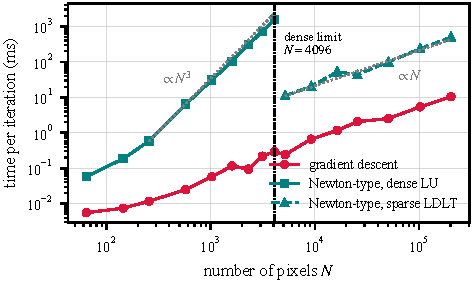
\includegraphics[width=\columnwidth]{scaling}
\caption{Wall time per iteration for Cameraman resampled to $n\times n$ pixels, $n$ from 8 to 450. The Newton-type method switches from dense LU to sparse $LDL^\top$ above $N=4096$.}
\label{fig:scaling}
\end{figure}

Fig.~\ref{fig:scaling} shows the cost of one iteration as the image grows. The dense path follows the $O(N^3)$ cost of LU: from $N=1024$ to $N=4096$ the time rises from 31\,ms to 1.61\,s, an exponent of 2.85. At the switch to the sparse solver the time drops by a factor of 145, to 11\,ms at $N=5184$. From there to $N=202{,}500$ the sparse path grows to 495\,ms, an observed exponent of 1.04, and GD from 0.24 to 10.4\,ms. At every size above the switch one NT iteration costs 20 to 50 GD iterations.

\section{Discussion}\label{sec:discussion}

For this problem the two methods trade iteration count against cost per iteration. NT needs about ten times fewer iterations to reach a given energy or its best PSNR, and its iterates settle quickly and monotonically, which makes stopping easy. GD is 22 to 35 times cheaper per iteration and reaches the same quality earlier in wall time at $225\times225$ pixels. Its progress depends on $L$ in \eqref{eq:lipschitz}: a small $\varepsilon$ or a large $\lambda$ slows it down, as the study at $\lambda=1$ shows.

The smoothing parameter matters more for NT than for GD, because the user can change it and because it trades bias for conditioning. With $\varepsilon=10^{-2}$ the bias is about 1\% of the energy and invisible in the images, but at $10^{-1}$ it is 14 to 19\%.

The results also show that the minimiser of the model is not the best denoised image. PSNR peaks after a few iterations at the default $\lambda$ and the methods only agree closely when $\lambda$ is chosen well. For a user, a $\lambda$ study is therefore more useful than running either method to high accuracy, and the application provides one.

The study has limitations. The PSNR-optimal $\lambda$ uses the clean image, which is unknown in practice. Timings depend on the sparse solver and memory hierarchy of one machine. Methods that avoid smoothing, such as Chambolle's projection algorithm \cite{chambolle2004}, FISTA \cite{beck2009} or the primal-dual algorithm of Chambolle and Pock \cite{chambolle2011}, were not compared.

\section{Conclusion}

Gradient descent with Armijo backtracking and the lagged diffusivity Newton-type method were implemented in a cross-platform C++ application and compared on identical seeded noise. At the PSNR-optimal $\lambda$ both give the same image quality within 0.08\,dB. The Newton-type method converges in far fewer iterations and decreases the smoothed objective monotonically, but each iteration needs a sparse factorisation that costs 20 to 50 gradient steps and its smoothing adds a bias of about 1\% in the exact energy. Gradient descent is faster in wall time for the image sizes studied, but slows down for large $\lambda$ or small $\varepsilon$. The dense Newton system becomes impractical beyond a few thousand pixels, while the sparse solver scales almost linearly up to 202{,}500 pixels.

\bibliographystyle{IEEEtran}
\bibliography{references}

\end{document}
